\documentclass[conference,letterpaper]{IEEEtran}
\usepackage{graphicx,amsmath,amssymb,booktabs,url,balance}
\usepackage[hidelinks]{hyperref}
\hyphenation{question-naire cali-bra-tion avail-ability}
\begin{document}
\title{Separating Recalibration from Retraining under Questionnaire Availability Shift: A BRFSS Stroke-History Study}
\author{\IEEEauthorblockN{Anonymous Authors}\IEEEauthorblockA{Research manuscript for review}}
\maketitle
\begin{abstract}
Missing questionnaire information can degrade probability predictions, but a fixed-model stress test cannot distinguish information loss from a mismatch between training and deployment inputs. We examine this distinction for self-reported stroke-history classification using public Behavioral Risk Factor Surveillance System data. Two model families, boosted trees and a multilayer perceptron, are evaluated under four predefined availability scenarios and four controls: global calibration, scenario-specific recalibration of a fixed full model, mixed-mask training, and subset retraining. All models use 2024 development data; the analysis protocol and model files are frozen before 2025 predictive evaluation. The 2025 file supplies 354,950 labeled respondents, including 16,353 positive histories. The primary common-jurisdiction comparison uses a three-seed probability ensemble and a survey-weighted paired Brier contrast. For demographics plus disease histories, mixed-mask boosted trees have lower Brier loss than scenario-recalibrated fixed models: -0.000157; the planned interval is unavailable because 93 strata contain only one PSU. Secondary analyses examine other feature sets, model families, and demographic domains. In severe availability scenarios, recalibration recovers much of the globally calibrated masked-model degradation, while further training gains depend on model family and scenario. This is an empirical methodological benchmark, not a new algorithm or prospective stroke prediction. Simulated information access, unweighted model fitting, and conditional survey-variance approximations limit interpretation.
\end{abstract}
\begin{IEEEkeywords}
stroke history, BRFSS, missing information, probability calibration, tabular learning, temporal transport
\end{IEEEkeywords}
\section{Introduction}
Stroke classification studies increasingly combine conventional classifiers, neural networks, and post-hoc explanations. Such tools can distinguish respondents with different reported health histories, but their reliability depends on what information is available at deployment. A classifier trained on demographic, behavioral, and disease-history variables may later receive only a subset. Replacing unavailable variables with an encoded missing state changes the predictor's input distribution; it does not reproduce training on that subset.

This distinction matters for claims of resource robustness. A poor score after masking a full model may reflect inappropriate deployment of that model, genuine loss of predictive information, or both. Probability recalibration is another possible remedy: a model can retain useful ranking while producing probabilities that are systematically too high or low. Comparing masked predictions only with full-information predictions cannot identify which remedy is needed.

We study these issues using the Behavioral Risk Factor Surveillance System (BRFSS), an annual cross-sectional telephone survey with public documentation and complex sampling weights \cite{cdc24,cdc25}. The endpoint is a respondent's report of ever being told by a health professional that they had a stroke. Current survey covariates do not necessarily precede that event. The task is therefore \emph{stroke-history classification}, not future stroke incidence prediction or acute diagnostic assessment.

Our empirical question is how much apparent availability degradation is corrected by recalibration and what further benefit known-pattern training or subset retraining provides. We separate four procedures under a common protocol, retain natural predictor nonresponse, and evaluate frozen 2024 models on the subsequent 2025 release. The primary contrast is declared before external scoring, and its uncertainty calculation uses survey strata and primary sampling units (PSUs).

The contributions are a controlled comparison of calibration and training remedies; a frozen survey-year transport evaluation with common-jurisdiction analysis; and an auditable separation of record-level predictive metrics from survey-weighted paired loss. We do not claim that mask-aware training, calibration, or subset refitting is algorithmically new. BRFSS is used as a population-health benchmark rather than evidence that an adaptive questionnaire should replace directly asking the stroke-history item.

\section{Related Work}
Ding \emph{et al.} analyzed NHANES and BRFSS questionnaire histories, comparing multiple classifiers with feature selection and SHAP \cite{ding}. Moulaei \emph{et al.} compared machine and deep learning with explainability in a smaller hospital dataset \cite{moulaei}. Their sampling, inputs, and endpoint settings differ from ours, so headline scores cannot establish superiority across studies. Strong tabular baselines also matter: boosted trees and carefully configured MLPs can be competitive without assuming that a more elaborate neural architecture must improve performance \cite{realmlp}.

Unavailable predictors and submodels are established topics. Janssen \emph{et al.} compared remedies for deliberately unavailable predictors, including submodels, and assessed calibration slope/intercept \cite{janssen}. Fletcher Mercaldo and Blume developed pattern submodels fitted within observed missingness patterns \cite{mercaldo}; our subset models instead use all eligible fitting respondents under a deliberately imposed availability set. Hoogland \emph{et al.} compare observed-predictor submodels, marginalization and imputation applicable to new individuals \cite{hoogland}. Sisk \emph{et al.} evaluate imputation and missing indicators across development and deployment \cite{sisk}.

Zhou \emph{et al.} formalize domain adaptation under missingness shift \cite{zhou}; Rockenschaub \emph{et al.} examine changing missingness mechanisms \cite{rock}. Deterministic known availability sets do not identify such mechanisms. Temporal validation and staged recalibration are established, as illustrated by Cooray \emph{et al.} \cite{cooray}. Our contribution is a matched four-procedure subsequent-year empirical comparison, not invention of its ingredients or a claim of priority over all prior studies. Reporting is informed by TRIPOD+AI \cite{tripod}.

\section{Data and Outcome}
\subsection{Cohorts and chronology}
The official 2024 XPT contains 457,670 records. Restricting the outcome to valid yes/no responses leaves 456,218 respondents, including 20,661 positive histories; 1,452 outcomes are excluded. We retain missing predictor values rather than selecting complete cases. The official 2025 release contains 356,158 records and 354,950 labeled respondents, including 16,353 positives. Table~\ref{tab:cohort} summarizes the executed analysis.

\begin{table}[t]
\caption{Executed cohorts and model-development partitions}
\label{tab:cohort}\centering\small
\begin{tabular}{lr}\toprule
Component & Respondents\\\midrule
2024 labeled source & 456,218\\
2024 fitting subset & 60,000\\
2024 stopping subset & 10,000\\
2024 calibration partition & 45,622\\
2024 development evaluation & 15,000\\
2025 labeled source & 354,950\\
2025 common-jurisdiction evaluation & 349,241\\
Common reporting jurisdictions & 49\\\bottomrule
\end{tabular}
\end{table}

The inherited 2024 split allocates 55/10/15/10/10\% to fitting, stopping, selection, calibration, and final testing. Stratified subsamples of the first three partitions provide the fitting, stopping, and development-evaluation sets in Table~\ref{tab:cohort}; the calibration partition is retained in full. Sampling uses fixed seeds. The remaining final-test partition is not newly scored in this study. Earlier work had already inspected 2024 test and 2023 transport results, so those observations are treated as exploratory for the final research direction.

Before 2025 predictive evaluation, we committed the availability protocol and froze model/source hashes. Inspecting the 2025 schema and official codebook established variable compatibility; no 2025 model fitting, calibration, or threshold selection was performed. Because reporting jurisdictions differ, the primary analysis restricts 2025 to the intersection with the 2024 source file. All-jurisdiction results are secondary. These are annual survey samples, not longitudinal follow-up of a patient cohort; anonymous respondent overlap cannot be checked.

\subsection{Predictors and availability}
The inherited 15 inputs comprise sex, age group, general health, exercise, smoking status, diabetes, myocardial infarction, coronary disease, kidney disease, arthritis, education, income, physically unhealthy days, mentally unhealthy days, and BMI. Survey weights, strata, PSU, and state are excluded from predictors. Valid outcome and missing-value codes are checked against both official codebooks. In particular, income codes 7 and 9 are valid categories, unhealthy-day code 88 denotes zero, and BMI has two implied decimal places.

Categorical missing values receive a separate imputed category; numeric inputs receive training-median imputation and missingness indicators, followed by standardization. All fitted preprocessing uses only the fitting respondents. For deliberately unavailable variables, the complete encoded block is zeroed and a separate availability indicator is set to zero. Natural nonresponse and deliberately unavailable questions therefore remain distinct operational states.

\begin{table}[t]
\caption{Predefined simulated availability sets}
\label{tab:sets}\centering\small
\begin{tabular}{p{.31\columnwidth}p{.59\columnwidth}}\toprule
Scenario & Retained information\\\midrule
Full (15) & All inherited predictors\\
Without health state (12) & Excludes general health and physically/mentally unhealthy days\\
Demographics + history (7) & Sex, age, diabetes, myocardial infarction, coronary disease, kidney disease, arthritis\\
Demographics (2) & Sex and age\\\bottomrule
\end{tabular}
\end{table}

Table~\ref{tab:sets} defines the four masks before scoring. The 12- and 7-variable sets are not nested, and feature count is not a validated acquisition cost. Removing current-health-state variables is a sensitivity analysis: remaining measurements can still postdate stroke or change after it. All four availability patterns are represented in mask training; this study tests year transport under known patterns, not generalization to arbitrary unseen masks.

\section{Experimental Protocol}
\subsection{Four controls}
Let $f$ be a full-input classifier, $M_s$ the encoding of scenario $s$, and $C_s$ a sigmoid calibration map fitted using 2024 calibration records under that scenario. We distinguish:
\begin{enumerate}
\item \emph{Fixed global calibration (FG):} $C_{\rm full}(f(M_s x))$. This exposes a full-trained, full-calibrated model to unavailable blocks.
\item \emph{Fixed scenario calibration (SC):} $C_s(f(M_s x))$. The classifier is unchanged; only a scenario-specific calibration map is fitted on 2024 data.
\item \emph{Mixed-mask training (MT):} a classifier trained on all four predefined masks, with a scenario-specific calibration map.
\item \emph{Subset retraining (SR):} a separate classifier and preprocessing pipeline fitted using only the retained predictors, followed by scenario-specific calibration.
\end{enumerate}
Each mask-trained fitting and stopping respondent appears once under each scenario with equal weight. These copies do not create new independent respondents. They increase optimization work relative to a single-scenario fit. The uniform mixture is an experimental choice, not an estimate of deployment frequency. In a full-trained model, availability flags are constant during fitting; the FG condition deliberately exposes the consequences of applying it outside those training conditions.

Sigmoid calibration uses logistic regression on a clipped probability logit with $C=1$. It is fitted independently of classifier training and stopping. Training and calibration are unweighted, with no class balancing or synthetic oversampling. Population weighting is applied in evaluation, so population calibration is not optimized directly during development.

\subsection{Model families and replication}
Histogram gradient boosting uses at most 200 iterations, learning rate 0.05, 31 leaves, and $L_2$ regularization 1. Early stopping uses the separate stopping partition with log-loss scoring and patience 15. The MLP uses hidden layers of 128 and 64 ReLU units, dropout 0.1 after the first hidden layer, and a sigmoid binary output. AdamW uses learning rate 0.001, weight decay 0.001, batch size 1,024, and 30 epochs; the minimum stopping binary cross-entropy checkpoint is retained.

Seeds 42, 43, and 44 share the same respondents and masks. No hyperparameter search is performed for this final experiment. Five classifiers per family/seed---full, mixed-mask, and three nonfull subsets---yield 30 fitted classifiers. Each family/scenario/condition uses the mean of its three calibrated seed probabilities as the primary ensemble prediction. Seed-specific results are also retained. The study does not claim exhaustive architecture optimization or equal wall-clock compute across procedures.

\subsection{Primary estimand and uncertainty}
The prespecified contrast compares MT with SC for boosted trees under demographics plus histories in the common-jurisdiction 2025 cohort. For respondent $i$, define
\begin{equation}
 d_i=(y_i-\bar p_{i,\mathrm{MT}})^2-(y_i-\bar p_{i,\mathrm{SC}})^2.
\end{equation}
Negative values favor MT. The survey-weighted ratio mean is
\begin{equation}
 \hat\theta=\frac{\sum_i w_i d_i}{\sum_i w_i},
\end{equation}
where $w_i$ is the final BRFSS weight. Strata are nested within state, and PSU totals are nested within those strata. With $m_h$ sampled PSUs in stratum $h$, define
\begin{align}
 t_{hg}&=\frac{\sum_{i\in(h,g)}w_i(d_i-\hat\theta)}{\sum_i w_i},\\
 \widehat V(\hat\theta)&=\sum_h\frac{m_h}{m_h-1}\sum_g(t_{hg}-\bar t_h)^2.
\end{align}
We use a with-replacement Taylor approximation, no finite-population correction, and a $t$ critical value with PSU-minus-strata degrees of freedom. No interval is returned if singleton strata prevent this calculation. For subgroup domains, outside-domain PSU contributions remain in the design with zero domain influence. The interval is conditional on the fitted models and does not capture training-sample uncertainty.

Secondary outcomes include unweighted and weighted Brier loss, AUROC, average precision (AP), negative log-likelihood (NLL), and unweighted ten-bin expected calibration error. AP is not trapezoidal area under a precision-recall curve. Brier is a proper probabilistic loss, not a pure calibration statistic. Other family/scenario contrasts and sex, age, and income domains are exploratory; no multiplicity-adjusted superiority claims are made. Domains require at least 200 respondents and 20 positives. Race/ethnicity is not analyzed, so this is not a comprehensive fairness assessment.

\section{Results}
\subsection{Frozen year transport}
The common-jurisdiction 2025 analysis contains 349,241 respondents and 16,082 positive histories across 49 reporting jurisdictions. No external refitting occurs. The primary weighted contrast is -0.000157; the planned interval is unavailable because 93 strata contain only one PSU. Thus MT has lower Brier loss than SC for the declared model/scenario. This statement is restricted to the executed estimand; statistical precision does not imply clinical utility or a new learning principle.

\begin{table}[t]\caption{2025 common-jurisdiction weighted metrics with seven available variables. Lower Brier is better.}\label{tab:primary}\centering\small
\begin{tabular}{llrrr}\toprule Family & Procedure & Brier & AP & AUROC\\\midrule
Trees & FG & 0.03322 & 0.1490 & 0.8044\\
Trees & SC & 0.03299 & 0.1490 & 0.8044\\
Trees & MT & 0.03284 & 0.1544 & 0.8114\\
Trees & SR & 0.03278 & 0.1577 & 0.8107\\
MLP & FG & 0.03721 & 0.1442 & 0.8048\\
MLP & SC & 0.03302 & 0.1442 & 0.8048\\
MLP & MT & 0.03279 & 0.1548 & 0.8121\\
MLP & SR & 0.03276 & 0.1578 & 0.8117\\
\bottomrule\end{tabular}\end{table}

Table~\ref{tab:primary} reports probability quality under the primary availability set for both families. All metric values come from saved predictions. Weighted AP and AUROC reflect the included weighted population; the model-fitting objective remains unweighted. For boosted trees in this scenario, global calibration gives Brier 0.03322, scenario calibration 0.03299, mixed-mask training 0.03284, and subset refitting 0.03278. FG--SC, SC--MT and MT--SR Brier reductions are 0.000227, 0.000157 and 0.000054. The primary reduction is approximately 0.48\% of SC Brier, without an established clinical benefit.

\begin{figure*}[t]\centering
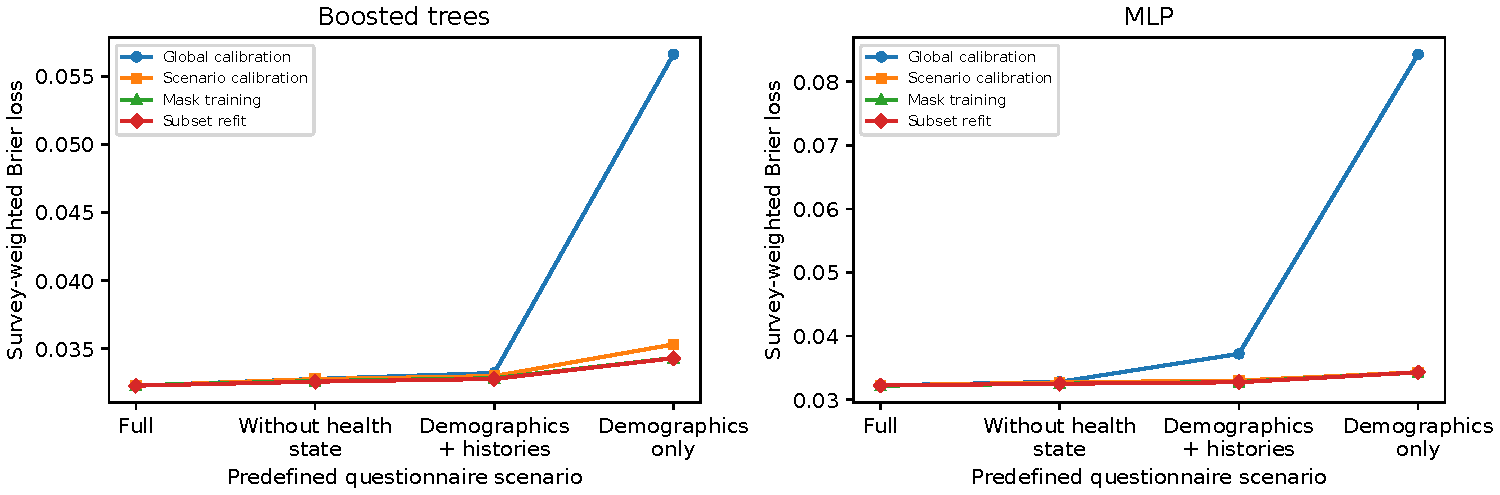
\includegraphics[width=.91\textwidth]{figures/availability.pdf}
\caption{Frozen 2025 common-jurisdiction performance across predefined availability sets. Lower Brier is better. The 12- and 7-variable sets are not nested; connecting lines distinguish procedures rather than imply a continuous resource budget. Each point uses a three-seed probability ensemble.}
\label{fig:availability}\end{figure*}

\subsection{Calibration and heterogeneity}
Figure~\ref{fig:calibration} shows survey-weighted reliability points in approximately equal-weight bins, keeping identical probabilities together. Post-hoc diagnostics of frozen predictions estimate calibration-in-the-large (CITL; logistic offset with slope fixed at one), joint logistic intercept/slope and weighted ECE. Ideal CITL/intercept/slope are 0/0/1. These diagnostic fits on 2025 outcomes are descriptive and never update deployed predictions. \begin{table}[t]\caption{Post-hoc weighted calibration diagnostics, seven-variable trees.}\centering\small\begin{tabular}{lrrrr}\toprule Procedure & CITL & Intercept & Slope & ECE\\\midrule FG & -0.333 & +0.485 & 1.333 & 0.0131\\
SC & +0.079 & +0.087 & 1.003 & 0.0029\\
MT & +0.055 & +0.119 & 1.023 & 0.0030\\
SR & +0.046 & +0.128 & 1.030 & 0.0029\\\bottomrule\end{tabular}\end{table} Scenario-specific recalibration is separated from classifier retraining, so the comparison cannot attribute every reduction in masked-model loss to improved feature representation. For seven-variable trees, FG has CITL $-0.333$ and slope 1.333 versus $+0.079$ and 1.003 for SC. MT has CITL $+0.055$ and slope 1.023; its lower Brier does not imply every calibration metric improves. For demographics-only trees, SC still has slope 0.719 versus 1.050 for MT. Demographics-only MLP Brier is nearly equal under SC and MT (0.03433 and 0.03430). Brier is not a pure calibration measure; additional training gains depend on model and scenario.

\begin{figure}[t]\centering
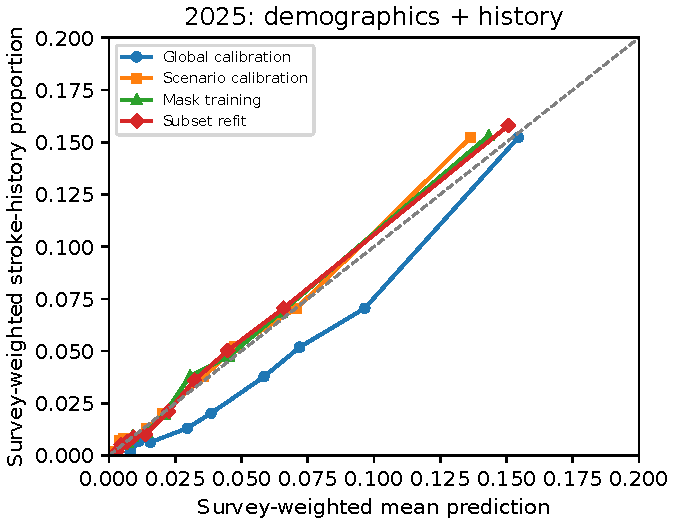
\includegraphics[width=.95\columnwidth]{figures/calibration.pdf}
\caption{Post-hoc survey-weighted calibration diagnostics of frozen seven-variable boosted-tree predictions. Prediction maps use 2024 data only.}
\label{fig:calibration}\end{figure}

The three seed-specific primary contrasts are -0.000156, -0.000148, -0.000160. Across the reported domains, weighted differences range from -0.000535 to -0.000040. Domain estimates concern the included respondents and cannot establish equal reliability across all demographic groups. The accompanying package provides the domain point-contrast figure; Fig.~\ref{fig:workflow} summarizes the original experiment. Domain intervals are also unavailable under the frozen singleton rule; no independent fairness tests are inferred. Full tables also include all 2025 jurisdictions and the common-jurisdiction 2024 development sample. Year-to-year metric differences are descriptive because prevalence and participant composition differ.

\begin{figure}[t]\centering\small
\fbox{\shortstack{2024 development respondents\\Separate fitting, stopping and calibration partitions}}\\[3pt]
$\Downarrow$\\[3pt]
\begin{tabular}{cc}
\fbox{\shortstack{FG: full classifier\\global calibration}} & \fbox{\shortstack{SC: same classifier\\scenario calibration}}\\[5pt]
\fbox{\shortstack{MT: shared classifier\\trained on four masks}} & \fbox{\shortstack{SR: separate classifiers\\for each feature subset}}
\end{tabular}\\[3pt]
$\Downarrow$\\[3pt]
\fbox{\shortstack{Freeze original models and calibration maps\\2025 common-jurisdiction evaluation\\Weighted paired Brier; discrimination and calibration}}
\caption{Original study workflow. All procedures use dedicated 2024 calibration data; each is evaluated under the same predefined availability sets. Post-hoc statistical diagnostics and fitting-sample checks are reported separately.}
\label{fig:workflow}\end{figure}

\section{Discussion}
The experiment separates three questions that a single robustness score can conflate: whether the full model tolerates a changed input representation, whether its probabilities can be recalibrated for that representation, and whether learning from partial inputs preserves information more effectively. The controls are operational procedure comparisons, not an identified causal or additive decomposition of independent mechanisms. The primary contrast measures training beyond recalibration. The protocol explicitly returns no interval when singleton strata prevent the planned variance calculation.

The point estimate is lower for mask-conditioned training beyond scenario recalibration in this cohort. However, the planned interval is unavailable and this is not a prespecified statistical-superiority finding. The absolute difference is a probability-loss contrast, not a clinical-effect estimate. Other masks and the MLP comparison are secondary. A favorable secondary result cannot replace the declared primary result.

Subset refitting provides a useful availability-specific reference, but it requires maintaining separate models. Mixed-mask training shares one classifier across the four known patterns, with separate calibration maps. Its practical attractiveness therefore depends on the accuracy/maintenance trade-off and the frequency of those patterns, neither of which is established by a uniform synthetic mask mixture. An arbitrary aggregate robustness index would obscure these choices; scenario-level proper scores provide the interpretable evidence in this study.

Probability quality should not be equated with comprehensive trustworthiness. This experiment does not jointly validate explanation stability, feature-level uncertainty attribution, or the utility of acquiring another question. Those are distinct empirical questions. In particular, dynamic-acquisition methods optimize a sequential decision problem, whereas the present study conditions on four fixed availability sets. No ranking against sequential acquisition algorithms is inferred from these results.

\section{Limitations and Reproducibility}
The endpoint is self-reported lifetime history. Current health, behavior, and comorbidity variables may be consequences of prior stroke; removing selected health-state inputs cannot restore temporal ordering. A respondent who can answer the target item can simply be asked directly. The study therefore does not validate diagnosis, prevention, or a clinically preferable adaptive questionnaire.

Only two model families, four known masks, one subsequent survey year, and a 60,000-person fitting subset are studied. Simulated unavailability is not evidence about real missing-not-at-random mechanisms. Conditioning on valid outcome responses can introduce selection effects. Different year coverage is addressed through a common-jurisdiction primary cohort, but it does not eliminate within-jurisdiction population changes. Unweighted fitting/calibration can differ from population-optimal procedures. The survey interval ignores model-fitting uncertainty and finite-population corrections; the singleton-stratum issue prevents the prespecified primary interval. Post-hoc survey sensitivities remain conditional on fitted models and cannot restore the unavailable prespecified interval. Neither broad algorithmic novelty nor state-of-the-art superiority is claimed.

This study reuses public CDC survey releases and recruits no participants; no additional participant contact or consent collection occurred. No institutional approval or exemption is asserted.

The repository contains the frozen configuration, official-data hashes, model manifest, training histories, aggregate tables, and figure-generation code. Participant-level data and predictions are excluded from tracked artifacts. The official releases are independently downloadable; private Drive-file byte identity is not assumed. The reproduction notebook has been syntax-checked, while account-specific Colab/Drive execution is not verified. All 35 automated tests pass. Frozen artifacts are checksum-verified; revision-specific audit records accompany the package. Editable manuscript source, analysis configuration and aggregate tables accompany this research draft.

\subsection{Post-evaluation survey-design audit}The full common-jurisdiction design contains 350,427 records before outcome restriction, versus 349,241 valid outcomes. Both have 2,034 strata and 93 single-PSU strata: outcome filtering did not create these singletons. A ratio-domain analysis retains zero influence outside valid outcomes while preserving their PSUs. Independent R survey4.2.1 execution reproduces the point estimate and fails to return an interval under the fail option. Separately labeled post-hoc sensitivities give 95\% t intervals (adjust: [-0.000254, -0.000059]; average: [-0.000256, -0.000057]). Adjust centers lonely contributions on the overall mean; average imputes the non-singleton mean contribution \cite{survey}. Python and R standard errors agree within numerical tolerance. These options require assumptions that cannot replace missing design information. The frozen primary interval remains unavailable; these are supportive sensitivities, not new confirmation. Models and deployed predictions are unchanged.

\subsection{Post-hoc fitting-sample robustness}Three new stratified 60,000-record draws from the original 2024 fitting pool (sampling seeds 2027--2029) retain fixed hyperparameters, stopping/calibration respondents and model seeds 42--44. Each uses full and mixed-mask classifiers to obtain a three-seed ensemble MT--SC contrast. Draws may overlap. Contrasts are -0.000163, -0.000040, -0.000175. All favor MT, but magnitudes vary substantially. These results assess sensitivity to fitting respondents conditional on the remaining fixed development choices; they are not survey-sampling intervals. The already-used 2025 cohort provides post-hoc robustness evidence, not fresh confirmation. All draws are reported without retuning.
\section{Conclusion}
A questionnaire-availability assessment should distinguish fixed-model masking, recalibration, mask-conditioned training, and subset refitting. Our frozen BRFSS year-transport experiment provides this comparison with a prespecified survey-weighted paired loss. The primary point estimate is lower for mixed-mask boosted trees in the seven-variable setting, but the planned interval is unavailable; no prespecified superiority claim is made. The evidence concerns self-reported stroke-history classification under simulated information access. It supports evaluating concrete deployment conditions and calibration controls rather than inferring trust from a single accuracy or robustness score.

\balance
\section*{AI Assistance Disclosure}
OpenAI ChatGPT assisted with analysis-code development and execution, literature synthesis, manuscript text and scientific figure-generation code throughout this study. Human authors remain responsible for verification, interpretation, final approval and submission.
\begin{thebibliography}{14}
\bibitem{cdc24} Centers for Disease Control and Prevention, ``2024 BRFSS survey data and documentation,'' 2025. [Online]. Available: \url{https://www.cdc.gov/brfss/annual_data/annual_2024.html}
\bibitem{cdc25} Centers for Disease Control and Prevention, ``2025 BRFSS survey data and documentation,'' 2026. [Online]. Available: \url{https://www.cdc.gov/brfss/annual_data/annual_2025.html}
\bibitem{ding} C. Ding, M. Yuan, J. Cheng, and J. Wen, ``Cross-sectional study on smoking types and stroke risk: development of a predictive model for identifying stroke risk,'' \emph{Frontiers in Physiology}, vol. 16, 2025, doi: 10.3389/fphys.2025.1528910.
\bibitem{moulaei} K. Moulaei \emph{et al.}, ``Explainable artificial intelligence for stroke prediction through comparison of deep learning and machine learning models,'' \emph{Scientific Reports}, vol. 14, art. 31392, 2024, doi: 10.1038/s41598-024-82931-5.
\bibitem{realmlp} D. Holzm\"uller, L. Grinsztajn, and I. Steinwart, ``Better by default: Strong pre-tuned MLPs and boosted trees on tabular data,'' in \emph{Advances in Neural Information Processing Systems}, vol. 37, 2024.
\bibitem{janssen} K. J. M. Janssen \emph{et al.}, ``Dealing with missing predictor values when applying clinical prediction models,'' \emph{Clinical Chemistry}, vol. 55, no. 5, pp. 994--1001, 2009, doi: 10.1373/clinchem.2008.115345.
\bibitem{mercaldo} S. Fletcher Mercaldo and J. D. Blume, ``Missing data and prediction: the pattern submodel,'' \emph{Biostatistics}, vol. 21, no. 2, pp. 236--252, 2020, doi: 10.1093/biostatistics/kxy040.
\bibitem{hoogland} J. Hoogland \emph{et al.}, ``Handling missing predictor values when validating and applying a prediction model to new patients,'' \emph{Statistics in Medicine}, vol. 39, pp. 3591--3607, 2020, doi: 10.1002/sim.8682.
\bibitem{sisk} R. Sisk \emph{et al.}, ``Imputation and missing indicators for handling missing data in the development and deployment of clinical prediction models: A simulation study,'' \emph{Statistical Methods in Medical Research}, vol. 32, no. 8, pp. 1461--1477, 2023, doi: 10.1177/09622802231165001.
\bibitem{zhou} H. Zhou, S. Balakrishnan, and Z. Lipton, ``Domain adaptation under missingness shift,'' in \emph{Proc. AISTATS}, PMLR, vol. 206, pp. 9577--9606, 2023.
\bibitem{rock} P. Rockenschaub \emph{et al.}, ``Robust prediction under missingness shifts,'' arXiv:2406.16484, 2024. [Preprint].
\bibitem{cooray} S. D. Cooray \emph{et al.}, ``Temporal validation and updating of a prediction model for the diagnosis of gestational diabetes mellitus,'' \emph{Journal of Clinical Epidemiology}, vol. 164, pp. 54--64, 2023, doi: 10.1016/j.jclinepi.2023.08.020.
\bibitem{tripod} G. S. Collins \emph{et al.}, ``TRIPOD+AI statement: updated guidance for reporting clinical prediction models that use regression or machine learning methods,'' \emph{BMJ}, vol. 385, e078378, 2024, doi: 10.1136/bmj-2023-078378.
\bibitem{survey} T. Lumley, ``Options for the survey package: handling singleton PSUs,'' \emph{survey} package documentation. [Online]. Available: \url{https://r-survey.r-forge.r-project.org/survey/html/surveyoptions.html}
\end{thebibliography}
\end{document}
